\documentclass[12pt,compress,ngerman]{beamer}
\usepackage{amsmath}
\usepackage{url}
\usepackage{ucs}
\usepackage[utf8x]{inputenc}
\usepackage[ngerman]{babel}
\usepackage{ulem}  % sout
\usepackage{multicol}

% Manual syntax highlighting
\newcommand{\synfunc}   [1]{\color{blue!50!black}#1\color{black}}
\newcommand{\synstr}    [1]{\color{red!50!black}#1\color{black}}
\newcommand{\synvar}    [1]{\color{purple!50!black}#1\color{black}}
\newcommand{\synclass}  [1]{\color{green!50!black}#1\color{black}}
\newcommand{\syncomment}[1]{\color{blue!20!black}#1\color{black}}
\newcommand{\syncool}   [1]{\color{beamer@blendedblue}#1\color{black}}
\newcommand{\synoder}      {\ \ \color{black}$\vee$\ \ }
\newcommand{\hr}        {\rule[4pt]{\textwidth}{0.1pt}\\}
\newcommand{\hicolor}   [1]{\color[rgb]{0.6,0.2,0.8}#1\color{black}}
\newcommand{\synhilight}[1]{\hicolor{\textbf{#1}}}

\newcommand{\synType}   [1]{\color{red!38!black}#1\color{black}}
\newcommand{\synSym}    [1]{\color{blue!56!black}#1\color{black}}
\newcommand{\synKey}    [1]{\color{blue!56!black}#1\color{black}}
\newcommand{\synLit}    [1]{\color{green!19!black}#1\color{black}}
\newcommand{\synOp}     [1]{\color{green!38!black}#1\color{black}}

\newcommand{\doofcomment}{\ \ \syncomment{\# :-(}}
\newcommand{\gutcomment} {\ \ \syncomment{\# :)}}

\newcommand{\T}[1]{\mathbf{#1}}
\newcommand{\Spur}[1]{\operatorname{Spur}{#1}}
\newcommand{\ul}[1]{\mathcal{#1}}

\newcommand{\floatbox}[3]{%
  \raisebox{0pt}[0pt][0pt]{%
    \begin{picture}(0,0)(#1,#2)#3\end{picture}%
  }%
}

\title{Haskell, \\eine rein funktionale Programmiersprache}
\author{Ingo Blechschmidt \\ \texttt{<iblech@web.de>}} % \\\texttt{<carina.willbold@student.uni-augsburg.de>}}
%\institute{{\footnotesize Universität Augsburg}}
\date{Augsburger Linux-Infotag 2010}

\usetheme{Warsaw}  %Warsaw, Berkeley?
\usecolortheme{seahorse}
\usefonttheme{serif}
\useinnertheme{rectangles}
\usepackage{bookman}
\setbeamercovered{invisible}

\setbeamertemplate{navigation symbols}{}
%\setbeamertemplate{headline}{}

\begin{document}

\frame{\titlepage}

\frame[plain]{\begin{center}
  
\includegraphics[scale=0.35]{images/learn-you-a-haskell-for-great-good.png}
\end{center}}

\section{Grundlegendes}
\frame[t]{\frametitle{Haskell ist komisch!}
  \floatbox{-210}{110}{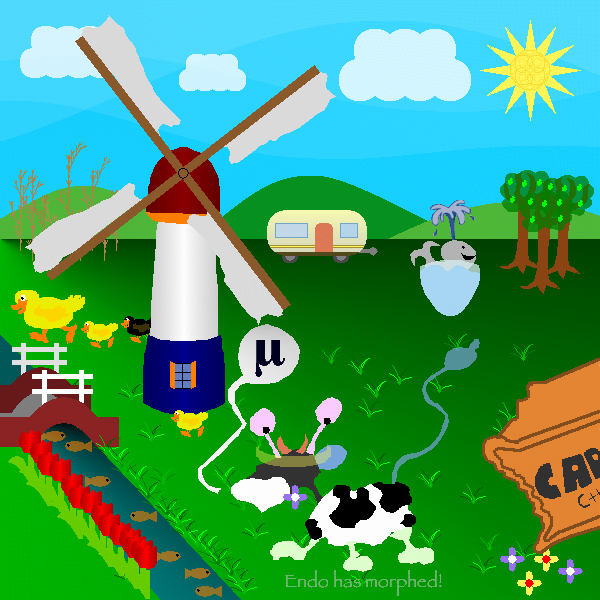
\includegraphics[scale=0.2]{images/endo.png}}%
  Haskell ist rein funktional:
  \begin{itemize}
    \item keine veränderliche Variablen
    \item keine Seiteneffekte
    \item keine Anweisungen
  \end{itemize}
}

\frame[t]{\frametitle{Bedarfsauswertung}
  \begin{minipage}{20cm}
    \texttt{%
      natürlicheZahlen \synSym{::}\ [\synType{Integer}] \\
      natürlicheZahlen \synSym{=}\ [\synLit{1}..] \\
      \ \\
      ungeradeZahlen \synSym{::}\ [\synType{Integer}] \\
      ungeradeZahlen \synSym{=}\ filter odd [\synLit{1}..] \\
      \ \\
      fibs \synSym{::}\ [\synType{Integer}] \\
      fibs \synSym{=}\ \synLit{0}\ \synOp{:}\ \synLit{1}\ \synOp{:}\ zipWith\ \synOp{(+)}\ fibs (tail fibs)
    }
  \end{minipage}
}

\frame[t]{\frametitle{Benutzerdefinierte Datentypen}
  \floatbox{-220}{190}{\scalebox{0.7}{\input{images/baum.pspdftex}}}%
  \texttt{%
    \synKey{data}\ \synType{Tree}\ = Leaf \synType{Int}\ | Fork \synType{Tree}\ \synType{Tree}
  }
  Konstruktoren: \\
  \texttt{Leaf \synSym{::}\, Int \synSym{->}\ Tree} und \\
  \texttt{Fork \synSym{::}\, Tree \synSym{->}\ Tree \synSym{->}\ Tree}

  \vfill
  \pause
  \texttt{%
    beispielBaum \synSym{=}\ Fork \\
    \ \ \ \ (Fork (Leaf \synLit{17}) (Leaf \synLit{37}))\\
    \ \ \ \ (Fork\\
    \ \ \ \ \ \ \ \ (Fork (Leaf \synLit{42}) (Leaf \synLit{0}))\\
    \ \ \ \ \ \ \ \ (Leaf \synLit{41}))
  }

  \vfill
  \pause
  \texttt{%
    komischerBaum \synSym{=}\ Fork \\
    \ \ \ \ (Fork (Leaf \synLit{23}) komischerBaum)
  }
}

\frame[t]{\frametitle{Benutzerdefinierte Datentypen (Forts.)}
  \floatbox{-223}{75}{\scalebox{0.7}{\input{images/baum.pspdftex}}}%
  \hspace*{-1em}\begin{minipage}{20cm}
  \texttt{%
    \synKey{data}\ \synType{Tree}\ \ \ = Leaf \synType{Int}\ | Fork \synType{Tree}\ \synType{Tree} \\
    \ \\
    \pause
    \synKey{data}\ \synType{Tree}\ a = Leaf a \ \ | Fork (\synType{Tree}\ a) (\synType{Tree}\ a)
    \pause
    \ \\
    \ \\
    size \synSym{::}\ \synType{Tree}\ a \synSym{->}\ \synType{Integer} \\
    size (Leaf \symbol{95})\ \ \ \ \ \ \ \ \ \ \ \ \synSym{=}\ \synLit{1} \\
    size (Fork links rechts) \synSym{=}\\
    \phantom{ }\ \ \ size links \synOp{+}\ size rechts
    \ \\
    \ \\
    \pause
    inorder \synSym{:}\ \synType{Tree}\ a \synSym{->}\ [a] \\
    inorder (Leaf x)\ \ \ \ \ \ \ \ \ \ \ \  \synSym{=}\ [x] \\
    inorder (Fork links rechts) \synSym{=} \\
    \phantom{ }\ \ \ inorder links \synOp{++}\ inorder rechts
  }
  \end{minipage}
}

\appendix
\section{Bildquellen}
\frame[t]{\frametitle{Bildquellen}
  \begin{itemize}
    \item \url{http://learnyouahaskell.com/splash.png}
    \item \url{http://save-endo.cs.uu.nl/target.png}
  \end{itemize}
}

\end{document}
